\documentclass[a4paper]{article}

%% Language and font encodings
\usepackage[english]{babel}
\usepackage[utf8x]{inputenc}
\usepackage[T1]{fontenc}
\usepackage{wrapfig}
\usepackage{subcaption}
\usepackage{graphics}
\usepackage{booktabs}
\usepackage{multirow}
\usepackage[table]{xcolor}
\usepackage{amsmath}
\usepackage{amsthm}
\usepackage{amsfonts}
\usepackage{tweaklist}
\usepackage{blindtext}
%% Useful packages
\usepackage{amsmath}
\usepackage{graphicx}
\usepackage[colorinlistoftodos]{todonotes}
\usepackage[colorlinks=true, allcolors=blue]{hyperref}
\usepackage{xeCJK}
\usepackage{listings}
%\usepackage{emumerates}
%% Sets page size and margins
\usepackage[a4paper,top=2cm,bottom=2cm,left=1cm,right=3cm,marginparwidth=2cm]{geometry}

% command for matrix inverse:
\newcommand \inv[1]{#1\raisebox{1.15ex}{$\scriptscriptstyle-\!1$}}

\begin{document}
\setlength{\leftskip}{20pt}
\title{VIO - Homework 2}
\author{YaoGeFAD,e-mail:{\it alexgecontrol@qq.com}}
\maketitle

%%%%% ------------------------ %%%%% 

% \begin{abstract}
% \end{abstract}
% \tableofcontents

%%%%--------------------------------------------------
% \clearpage

\subsection*{说明:} %Enter instruction text here
\begin{itemize} 
\item 文本使用在线\LaTeX 编辑器 \url{https://www.overleaf.com}生成
\end{itemize}
\line(1,0){350}

\begin{enumerate} %starts the numbering
    \item[1.] {\bf Allan方差标定曲线生成}
    设置IMU仿真代码中不同的参数,生成Allan方差标定曲线:

    \item[$\ast$]{\bf ANS:}
    
    使用工具\textbf{\href{https://github.com/gaowenliang/imu\_utils}{imu\_utils}}生成Allan方差标定曲线流程如下:
    \begin{enumerate}
        \item 修改ROS版vio\_data\_simulation中src/gener\_alldata.cpp文件中的输出路径,使其与系统文件路径相匹配.
        \item 在标准版vio\_data\_simulation中src/imu.cpp文件中实现两种积分方法,编译,并使用python\_tool下draw\_trajectory.py文件验证实现的正确性.
        \item 将前述两积分实现移植到ROS版本中.
        \item 设置src/param.h下的IMU参数,使用ROS版本vio\_data\_simulation生成ROS bag.
        \item 首先加入Package code\_utils进行编译, 随后再加入imu\_utils进行编译.
        \item 修复code\_utils中头文件引用错误\href{https://github.com/AlexGeControl/Auto-Car-03-SLAM-00-Algorithms/blob/master/08-imu/ros/code_utils/src/sumpixel_test.cpp}{sumpixel\_test.cpp}
        \item 使用imu\_utils分析所得的ROS bag,绘制Allan variance curve.
    \end{enumerate}    

    为了不使用MATLAB的绘图功能,首先使用Python将工具所提供的\href{https://github.com/AlexGeControl/Auto-Car-03-SLAM-00-Algorithms/blob/master/08-imu/ros/imu_utils/scripts/draw_allan.py}{draw\_allan.m}重新实现.\textbf{具体实现细节请参考链接所指向的GitHub Repo}.
    
    使用中值积分进行IMU仿真,所得的Allan方差曲线如图\ref{fig:allan}所示. 该图片已同步到GitHub Repo,可通过上述Python脚本工具复现:
    \begin{figure}[h]
        \centering
        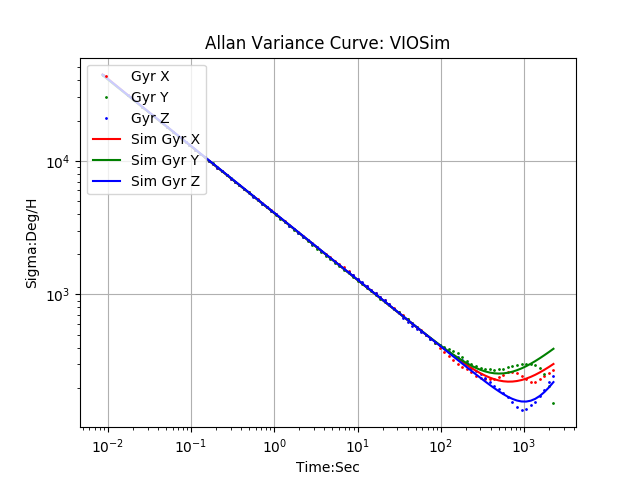
\includegraphics[width=0.618\textwidth]{viosim-allan-variance-curve}
        \caption{Allan Variance Curve for VIO Sim IMU @ 200Hz}
        \label{fig:allan}
    \end{figure}
    
    \textbf{相应的YAML文件请参考}\href{https://github.com/AlexGeControl/Auto-Car-03-SLAM-00-Algorithms/blob/master/08-imu/ros/imu_utils/data/VIOSim_imu_param.yaml}{VIOSim\_imu\_param.yaml}
    
    \item[2.]{\bf 中值积分的实现}
    将IMU仿真代码中的欧拉积分替换成中值积分

    \item[$\ast$]{\bf ANS:}
    中值积分的C++实现如下. \textbf{请参考链接所指向的GitHub Repo链接以获取具体实现细节}
    \begin{enumerate}
        \item \href{https://github.com/AlexGeControl/Auto-Car-03-SLAM-00-Algorithms/blob/master/08-imu/standard/src/imu.cpp}{\textbf{Standard} Version}.
        \item \href{https://github.com/AlexGeControl/Auto-Car-03-SLAM-00-Algorithms/blob/master/08-imu/ros/vio_data_simulation/src/imu.cpp}{\textbf{ROS} Version}.
    \end{enumerate} 

    实现时对参考代码进行了重构,将欧拉积分与中值积分全部封装为函数,同时依靠宏定义,使具体实现可在编译时通过宏指定.

    使用欧拉积分进行IMU仿真,所得的Trajectory曲线如图\ref{fig:euler}所示.
    \begin{figure}[h]
        \centering
        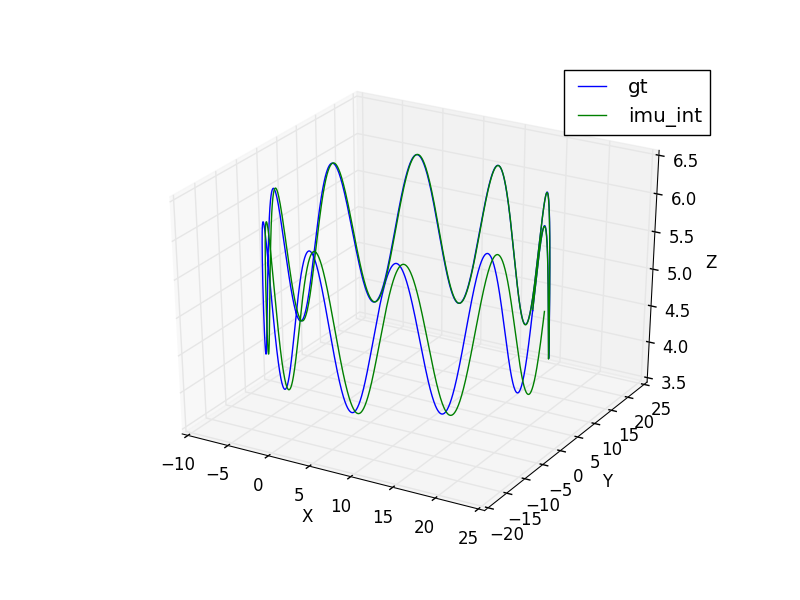
\includegraphics[width=0.618\textwidth]{viosim-trajectory-euler}
        \caption{Trajectory using Euler Integration}
        \label{fig:euler}
    \end{figure}

    使用中值积分进行IMU仿真,所得的Trajectory曲线如图\ref{fig:midpoint}所示.
    \begin{figure}[h]
        \centering
        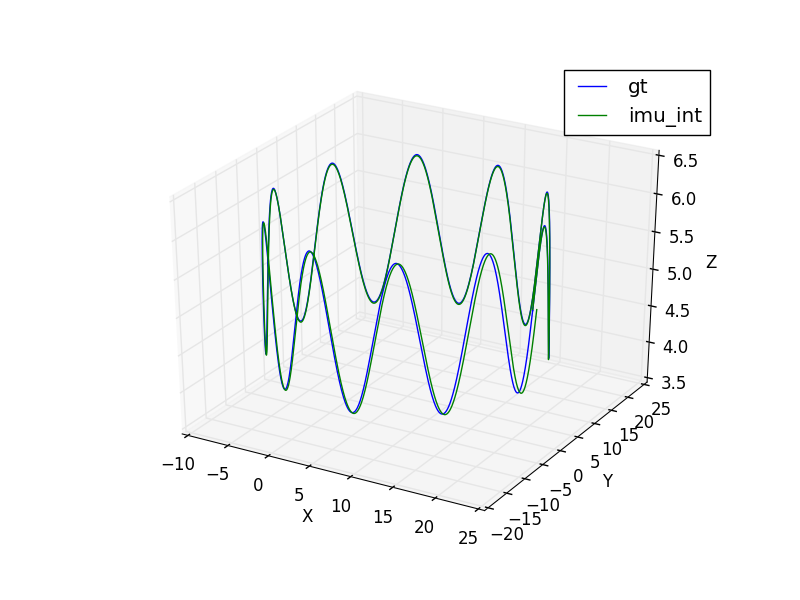
\includegraphics[width=0.618\textwidth]{viosim-trajectory-midpoint}
        \caption{Trajectory using Euler Integration}
        \label{fig:midpoint}
    \end{figure}
\end{enumerate}
% ends the numbering
\newpage

% -----------------------------------Appendix----------------------------------------
% -----------------------------------REFERENCE----------------------------------------
\begin{thebibliography}{9}

\bibitem{vionet}
Steven Lovegrove (2013) \emph{Spline Fusion: A Continuous-Time Representation for Visual Inertial Fusion with Application to Rolling Shutter Camera}, BMVC.

\end{thebibliography}

\end{document}